\documentclass[11pt]{article}
\usepackage[margin=1in]{geometry}
\usepackage{amsmath,amssymb}
\usepackage{booktabs}
\usepackage{graphicx}
\usepackage{hyperref}
\usepackage[T1]{fontenc}
\newcommand{\code}[1]{\texttt{#1}}
\title{fmix Layer 2: A Best-Effort Size Contract for Phase A\\
\large Mechanism, Controller Design, and the Running Experiments}
\author{local\_mixing working notes}
\date{2026-07-31}

\begin{document}
\maketitle

\begin{abstract}
Layer 2 turns phase A from a set of hand-tuned rates into a \emph{contract}:
a caller states a size trajectory --- expand to $R_1\times$ the input by
$N_0$ units of effective work, hold until $N_1$, compress toward
$R_2\times$ within a further budget --- and a controller delivers it, or
says clearly why it cannot. The single lever is \code{p\_mix}, the per-round
MIX/COMP coin; the controller identifies the plant from the monitors the
run already keeps, and steers. Crucially it does \emph{not} model twists:
it measures their effect as a disturbance, which is what lets a profile run
at any twist rate without being told the rate. This note gives the
mechanism, the design decisions (especially the anti-over-steer measures),
what validation established, and the eight-arm experiment now running on a
100k-gate, 512-wire slice. Headline from the runs so far: the four
$R_1$ arms track their setpoints inside $\pm 3\%$ across expansion and
hold, and there is a hard \emph{twist ceiling} --- at
\code{p\_twist}~$=5\times10^{-3}$ no size contract is achievable at any
lever setting.
\end{abstract}

\section{What layer 2 is}

\subsection{The phase-A defaults (\code{--phase-a})}

A single flag fixes the phase-A operating point: g57-word twist brackets
(\code{--twist-g57}) at \code{p\_twist}~$=5\times10^{-4}$;
\code{--db-advance} on (per the standing directive --- DB splice products
must ride their assigned direction); equal parts convex and contiguous
window sampling (\code{p\_convex}~$=0.5$); MIX with
\code{p\_mingen}~$=0.6$ and the curated cascade
(\code{--curated}, \code{--mix-pay-random}); COMP with
\code{p\_mingen}~$=0$ and the regular store only. Any flag given
explicitly on the command line wins, and the startup banner prints the
\emph{resolved} values, so a run states what it actually is.

\textbf{\code{--mix-pay-random}} is the one selection change: when a MIX
window's store answer contains only \emph{larger} spellings, take a
uniformly random one rather than a minimal one. This buys growth and
spelling diversity per paid splice --- and gives the controller a stronger
up-lever.

\subsection{The size profile (\code{--profile N0,N1,N2,R1,R2})}

Three phases, in effective-work units $E$ (cumulative moves per gate ---
the same clock all our analysis uses, so the contract is size-independent):

\begin{enumerate}
\item \textbf{expand} to $R_1 \cdot S_{\text{in}}$ by $E = N_0$;
\item \textbf{hold} near $R_1 \cdot S_{\text{in}}$ until $E = N_1$;
\item \textbf{compress} toward $R_2 \cdot S_{\text{in}}$, ending on arrival
or at $N_2$ --- whichever comes first.
\end{enumerate}

The setpoint $S^*(E)$ is the corresponding piecewise-linear trajectory.
$N_2$ may be an absolute mark ($N_2 \ge N_1$) or the compression leg's
\emph{budget}; a value below $N_1$ can only mean the latter, and the run
logs the absolute end mark it derived. A completed schedule \emph{ends the
run} (\code{MixStop::ProfileDone}) rather than burning the remaining move
budget outside any setpoint --- which, at a twist rate the lever cannot
offset, actively undoes the compression leg (measured: $+309\%$ over target
before this stop existed).

\subsection{One size authority}

\code{fmix} previously had three mechanisms pushing size around --- the
thermostat's static \code{target\_size}, the size brake's
\code{size\_hi}/\code{size\_lo} guard rails, and the \code{p\_mix} coin.
Adding a controller as a fourth would have produced two controllers on one
plant: the profile pressing the accelerator through phase 1 while the brake
(seeing ``runaway growth'') and the thermostat (still targeting the input
size) pressed back --- and the plant estimates would have been polluted by
their interference. So while a profile is active it is the \emph{only} size
authority: it owns \code{target\_size}, continuously setting it to
$S^*(E)$ so the thermostat is conscripted rather than disabled, and the
static brake is inert. Passing \code{--target-size}, \code{--size-hi},
\code{--size-lo} or \code{--p-mix} alongside \code{--profile} is refused
outright rather than silently overridden.

\section{The controller}

\subsection{Plant identification}

Every \code{--prof-cadence-eff} of effective work (default $0.5$) the
controller reads the run's own counters and estimates three quantities, all
in \emph{gates per move}:

\begin{itemize}
\item $\hat g$ --- drift if the lever were pinned at $1$ (all MIX);
\item $\hat s$ --- removal rate if the lever were pinned at $0$ (all COMP);
\item $\hat d$ --- the \textbf{disturbance}: the residual between the
observed total drift and the drift the DB move accounts for.
\end{itemize}

$\hat g$ and $\hat s$ come from per-mode gate-delta counters added for this
purpose, normalised by the lever actually in force over the interval (an
arm that saw too little of the interval keeps its previous estimate rather
than dividing by $\approx 0$). All three are EWMA-smoothed
(\code{--prof-ewma}).

\subsection{Why the disturbance term is the whole trick}

The controller cannot steer the twist rate --- twists are a layer-1
mechanism with their own purpose --- so it must \emph{cope} with it. Rather
than modelling twist growth (which would need the rate, the bracket cost,
the absorption statistics\ldots), the controller measures what it does:
everything that changes size and is not the DB move lands in $\hat d$.
Twists dominate that residual; expansion moves and thermostat contractions
also live there. The lever then solves
\[
p\,\hat g \;-\; (1-p)\,\hat s \;+\; \hat d \;=\; v^*,
\]
where $v^*$ is the slope that lands on the setpoint one cadence ahead, plus
a small integral term on the tracking error. A twist-heavy run simply gets
a lower \code{p\_mix}, automatically, with no knowledge of the twist rate.

The running experiments validate the mechanism directly:
$\hat d = +0.0000$ with twists off, $+0.0042$ at
\code{p\_twist}~$=5\times10^{-4}$, $+0.0388$ at $5\times10^{-3}$.

\subsection{Not over-sampling, not over-steering}

Measurement is $O(1)$ counter reads --- there is no census cost --- so
``over-sampling'' is purely a statistical concern, addressed by the cadence
and the EWMA. Over-steering is the real risk, and four guards address it:

\begin{itemize}
\item \textbf{cadence in effective-work units}, so control frequency scales
with circuit size and each interval contains tens of thousands of rounds;
\item \textbf{deadband} (\code{--prof-deadband}, default $2\%$): no lever
change while the size is close to setpoint;
\item \textbf{rate limit} (\code{--prof-dp-max}, default $0.1$ per update)
--- with an \emph{escape hatch}: the limit is lifted while more than four
deadbands from the setpoint, because a $0.1$-per-step crawl cannot catch a
ramp only six effective-work units long. Gentle where gentleness matters,
free where it does not;
\item \textbf{phase hysteresis}: the integral term and saturation counter
reset at each phase boundary.
\end{itemize}

\subsection{Best effort, stated honestly}

Not every profile is reachable. When the lever pins and the size is still
clearly off setpoint, the controller logs \code{profile: SATURATED} and
holds the pinned lever --- it does not thrash, and it does not abort. Phase
3 additionally diagnoses the specific infeasibility that matters:
when $\hat d > \hat s$, the disturbance exceeds the maximum available
removal, so the circuit grows with the lever at $0$ no matter what, and the
log says exactly that (\emph{lower the twist rate or relax $R_2$}). Every
control point prints \code{phase}, \code{eff}, \code{size}, $S^*$,
\code{pmix}, $\hat g$, $\hat s$, $\hat d$, the integrator and the
saturation counter, so a run's adherence to its contract is auditable after
the fact.

\section{What validation established}

\subsection{The plant}

On the 100k gadget at the phase-A operating point: $\hat g \approx 1.7$--$1.8$
gates/move at full lever --- consistent with the parallel session's
independent \code{p\_mix} sweep (final size ratio $1.28\times \to 3.27\times$
over \code{p\_mix} $0.05 \to 0.40$, monotone and smooth). Critically,
$\hat s$ \emph{decays} as material hardens: from $\approx 0.5$ early to
$\approx 0.005$ late in a 20k run. A static feed-forward table calibrated on
early drift would therefore overshoot badly late in a run --- live
estimation is not a refinement here, it is a requirement.

\subsection{Two defects the first runs exposed}

\textbf{Early overshoot.} A \code{p\_mix}$=1.0$ prior blew past the
expansion ramp before the first update (measured $185$k against a $118$k
setpoint). Fixed by a moderate $0.5$ prior, a first update at quarter
cadence, and the escape hatch above.

\textbf{Idling past completion.} Without the profile-complete stop, a
finished schedule kept mixing outside any setpoint; at a twist rate the
lever could not offset, it grew to $+309\%$ over target.

\subsection{Two preset defects found by reading a live banner}

\code{--phase-a} decided ``did the user specify this?'' by comparing each
knob to its default \emph{value}, so \code{--p-twist 0} --- a real request,
and also the default --- was silently overwritten with $5\times10^{-4}$: an
intended no-twist arm ran as an exact duplicate of its baseline. It now
keys on whether the flag appeared on the command line. Separately,
\code{p\_mingen} ships at $0.8$, not the $0.6$ phase A calls for, and a
stale comment led the preset to skip setting it. Both fixed; the banner now
prints resolved values.

\section{The running experiments}

Eight arms, all from the same 100k-gate, 512-wire slice, sampled ancestry
($K = 256$), measurements every 200k moves. Four are the requested $R_1$
sweep; four isolate one axis each against the \code{nR20} baseline.

\begin{table}[h]\centering\small
\begin{tabular}{llll}
\toprule
arm & profile & \code{p\_twist} & what it isolates \\
\midrule
\code{nR15} & $5,50,+20,\;1.5,1.2$ & $5\!\times\!10^{-4}$ & expansion ratio \\
\code{nR20} & $5,50,+20,\;2.0,1.2$ & $5\!\times\!10^{-4}$ & baseline \\
\code{nR25} & $5,50,+20,\;2.5,1.2$ & $5\!\times\!10^{-4}$ & expansion ratio \\
\code{nR30} & $5,50,+20,\;3.0,1.2$ & $5\!\times\!10^{-4}$ & expansion ratio \\
\code{notwist} & $5,50,+20,\;2.0,1.2$ & $0$ & twist axis \\
\code{nR20\_tw5} & $5,50,+20,\;2.0,1.2$ & $5\!\times\!10^{-3}$ & twist axis \\
\code{nR20\_fast} & $5,20,+20,\;2.0,1.2$ & $5\!\times\!10^{-4}$ & hold duration \\
\code{nR20\_slow} & $5,100,+20,\;2.0,1.2$ & $5\!\times\!10^{-4}$ & hold duration \\
\bottomrule
\end{tabular}
\caption{The question is which shape buys the most mixing quality per unit
of work --- read from the sampled-ancestry measures (\code{desc},
\code{cov}, \code{ent}) along the way and from affine-reconstruction plates
on the finals.}
\end{table}

\subsection{Tracking, in progress}

\begin{center}\small
\begin{tabular}{lrrrrrr}
\toprule
arm & phase & $E$ & size & $S^*$ & error & \code{p\_mix} \\
\midrule
\code{nR15} & hold & 42.2 & 147{,}766 & 150{,}000 & $-1.5\%$ & 0.000 \\
\code{nR20} & hold & 28.2 & 193{,}975 & 200{,}000 & $-3.0\%$ & 0.091 \\
\code{nR25} & hold & 22.2 & 245{,}538 & 250{,}000 & $-1.8\%$ & 0.111 \\
\code{nR30} & hold & 18.3 & 295{,}169 & 300{,}000 & $-1.6\%$ & 0.085 \\
\code{nR20\_slow} & hold & 28.2 & 193{,}975 & 200{,}000 & $-3.0\%$ & 0.091 \\
\code{nR20\_fast} & compress & 28.9 & 168{,}584 & 164{,}473 & $+2.5\%$ & 0.000 \\
\code{nR20\_tw5} & hold & 39.1 & 368{,}552 & 200{,}000 & $\mathbf{+84\%}$ & 0.000 \\
\bottomrule
\end{tabular}
\end{center}

Six of seven track inside $\pm 3\%$, including \code{nR20\_fast} descending
its compression ramp. (\code{nR20} and \code{nR20\_slow} agree exactly:
same seed, and their setpoints coincide until $E = 50$ --- a useful
determinism check.)

\subsection{The twist ceiling}

\code{nR20\_tw5} is the informative failure. At
\code{p\_twist}~$=5\times10^{-3}$ the controller cannot even \emph{hold}:
the lever is pinned at $0$ and the circuit still runs $84\%$ above
setpoint, because $\hat d = +0.039$ gates/move exceeds the maximum
available removal $\hat s = +0.021$. This reproduces a 20k-scale result
exactly, and it is a genuine constraint rather than a controller
deficiency: \textbf{a size contract and a high twist rate are mutually
exclusive}. Choose the twist rate first, then ask for a profile the plant
can deliver.

\begin{figure}[h]\centering
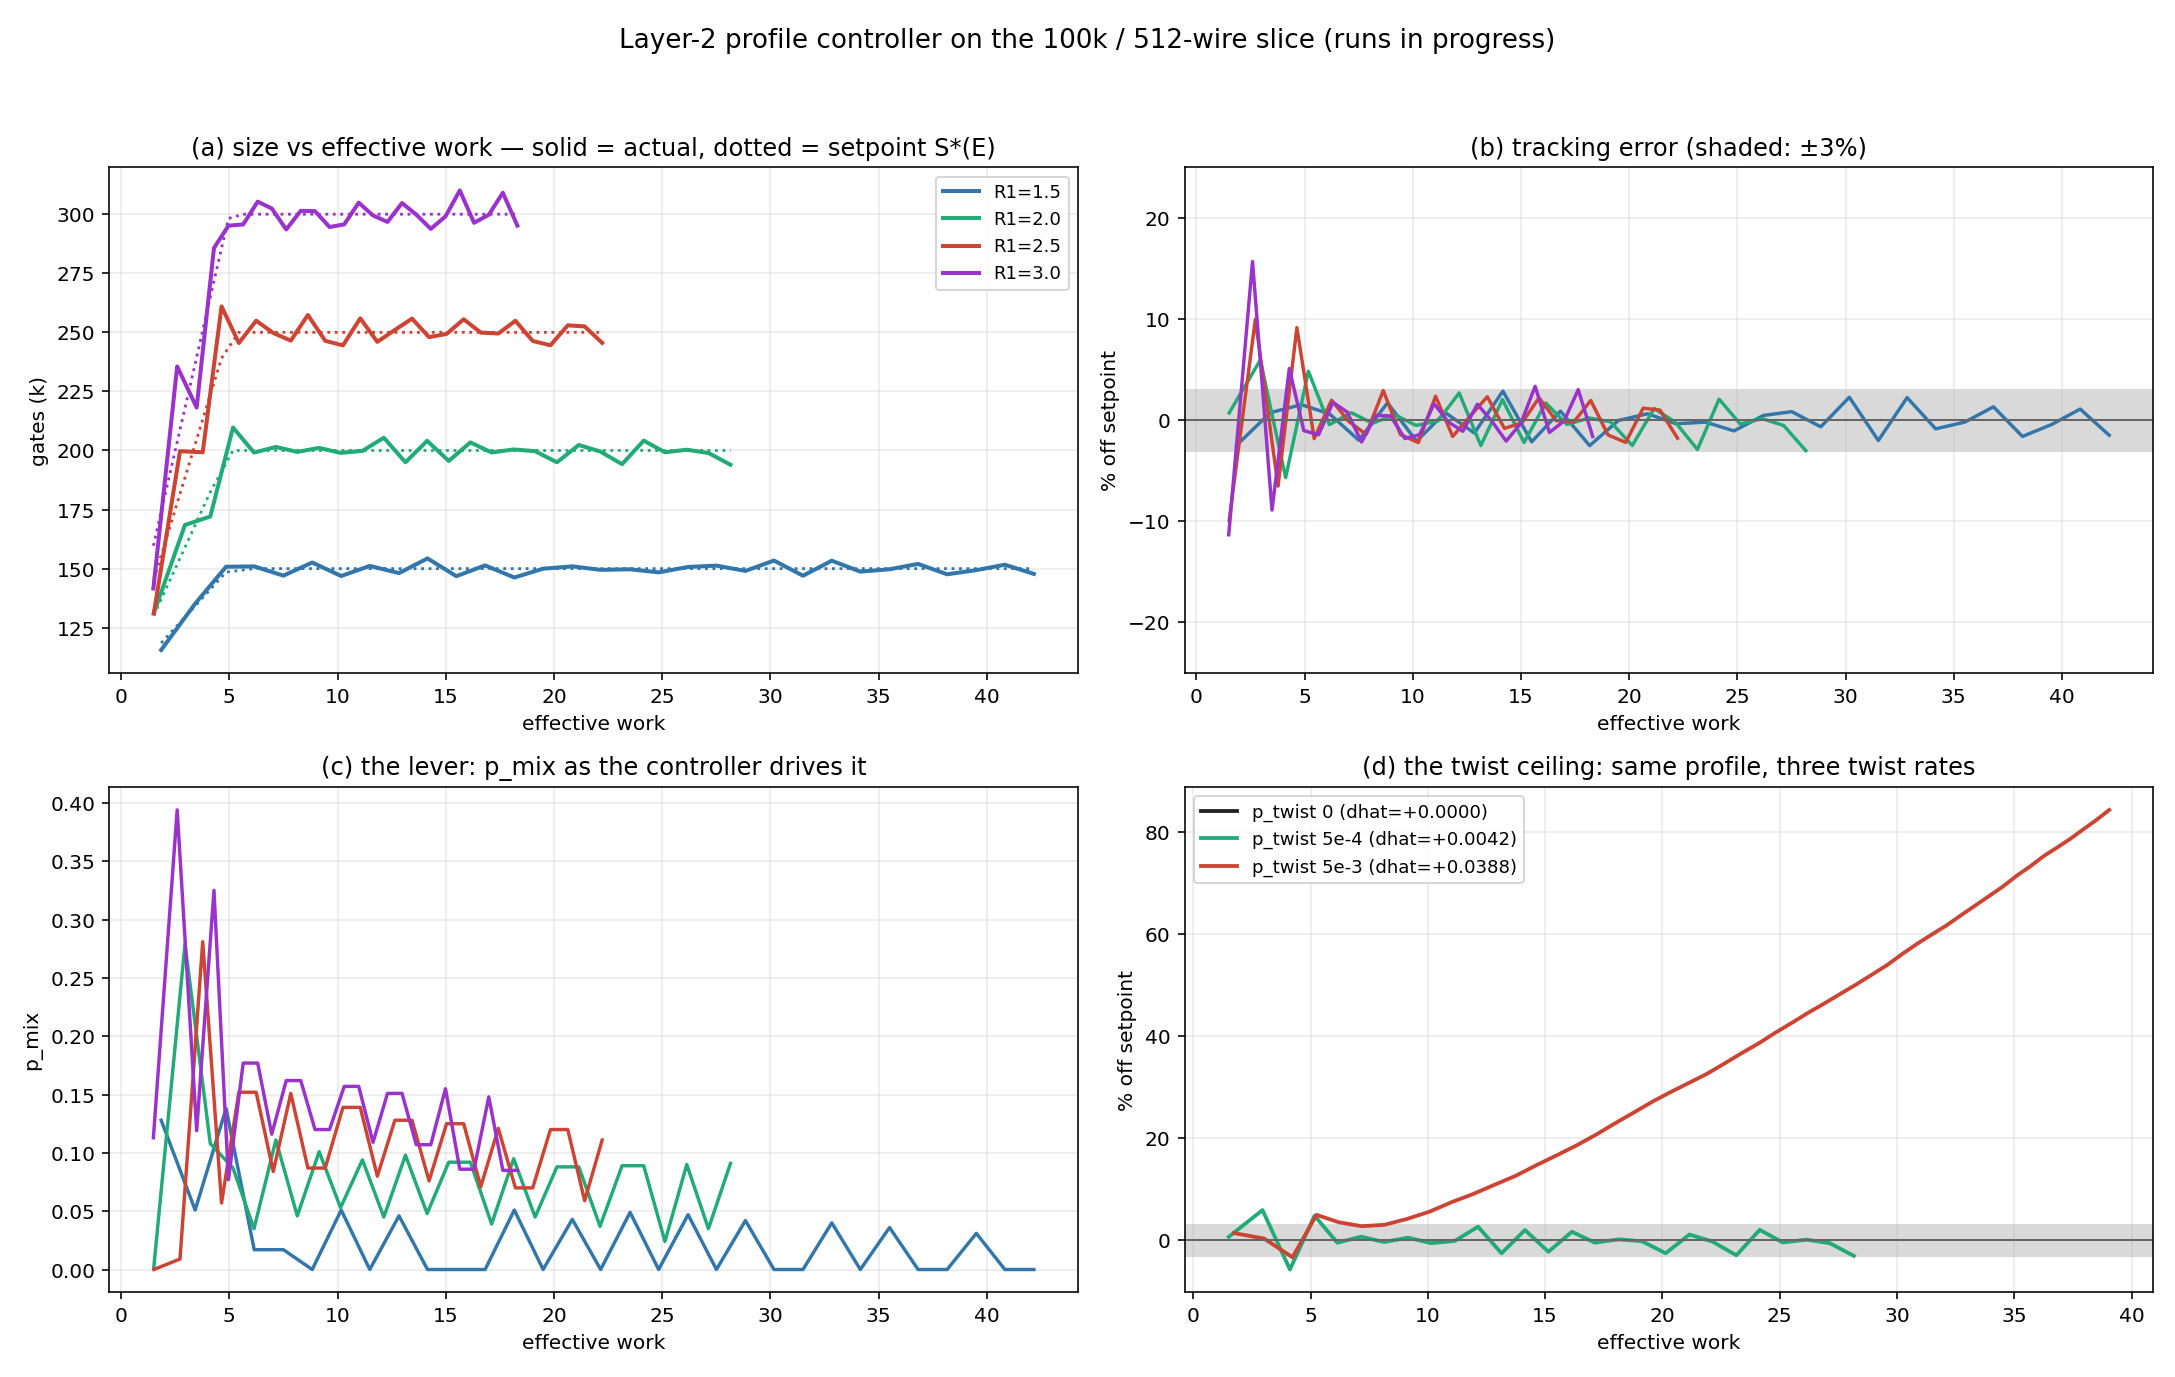
\includegraphics[width=\textwidth]{../reports/ancestry_20260728/layer2_tracking_20260731.png}
\caption{(a) size against effective work, actual (solid) versus setpoint
(dotted), for the four $R_1$ arms; (b) tracking error, shaded band
$\pm 3\%$; (c) the lever the controller chose; (d) the twist axis --- same
profile at three twist rates, with the measured disturbance in the legend.}
\end{figure}

\section{Caveats and open items}

\begin{itemize}
\item The running arms use \code{p\_mingen}~$=0.8$, not the phase-A
$0.6$, because the preset defect above was found after they launched. Every
arm shares it, so the \emph{comparison between profiles} is sound; the
absolute operating point is not exactly phase A. The intended remedy is to
rerun only the winning profile at the exact spec.
\item A profile is a whole-run construct: its effective-work clock is not
serialised, so \code{--profile} on a \code{--resume} restarts the schedule
at $E = 0$ (warned at startup).
\item Single trajectories, one seed per arm --- these are engineering
measurements, not replicated statistics.
\item The mixing-quality comparison (which profile shape is best) is the
point of the campaign and is still pending: the arms are mid-flight.
\end{itemize}

\end{document}
